\documentclass{article}

\usepackage{fullpage}
\usepackage{graphicx}


\title{Práctica 7: Rectificación mediante diodos}
\date{}
\author{Pablo Cuesta Sierra. Grupo 1201. Puesto 10.}



\begin{document}

\maketitle

\begin{center}
\section*{Montaje experimental}
\end{center}

\textbf{Construya el Circuito 1 utilizando los diodos suministrados. La señal de V1 se obtendrá
del generador de funciones, mientras que las fuentes V2 y V3 serán las fuentes S1 y S2 de la
fuente de alimentación disponible en el laboratorio. Es importante notar que el terminal positivo
de V3 se conecta a masa y que la señal a conectar al diodo D2 se extrae del terminal negativo,
al revés de lo que ocurre para V2.}

\bigskip
\begin{center}
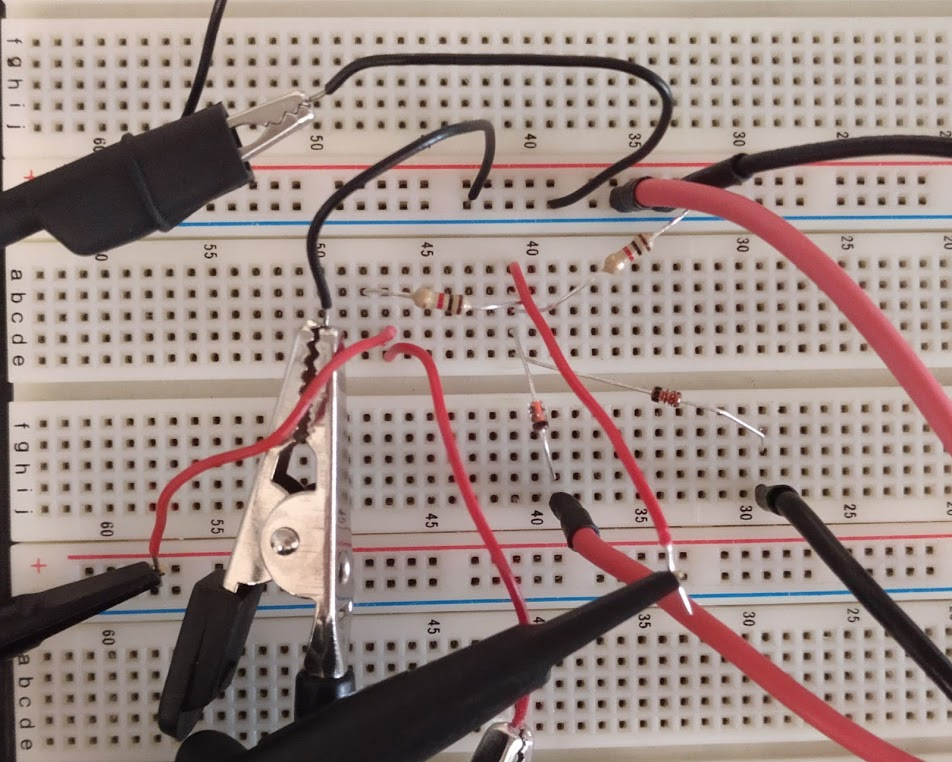
\includegraphics[scale=0.2]{c1}\\
Circuito 1 montado en la entrenadora.
\end{center}


\textbf{a) Genere para V1 una señal sinusoidal de 5 voltios de amplitud y 5 KHz de frecuencia.
Fije las tensiones de V2 y V3 en 1.2 V y 0.7 V, respectivamente. Mida la señal de
salida y determine experimentalmente las tensiones umbral de los diodos
suministrados. }

\bigskip
\begin{center}
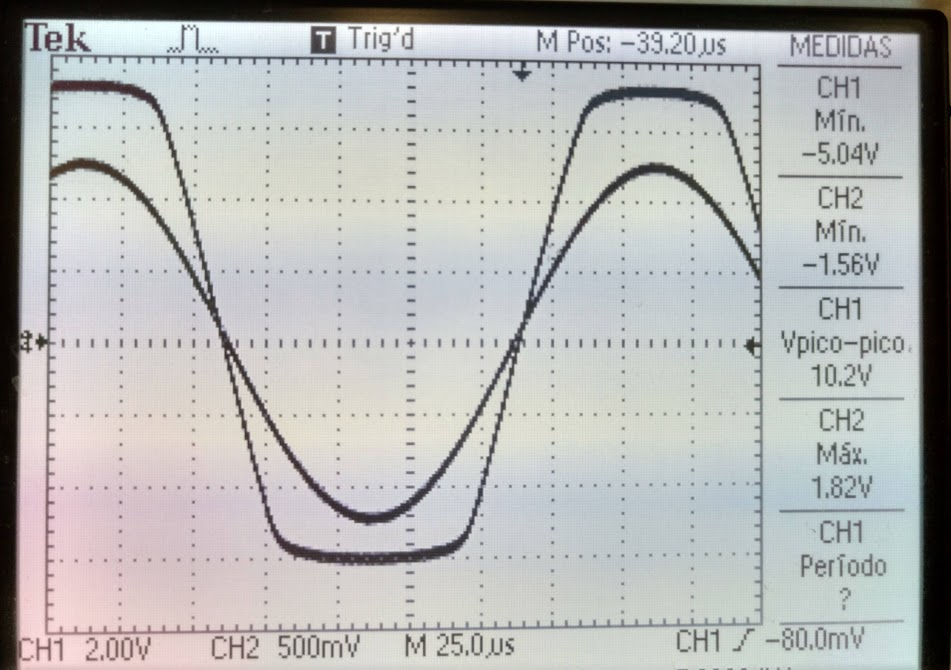
\includegraphics[scale=0.2]{med1}\\
Medidas hechas en el osciloscopio para el Circuito 1.
\end{center}

Como podemos ver en la imagen anterior (medidas correspondientes al CH2), $V_{out, max}=1,82V$ y $V_{out, min}=-1,56V$, además, la función obtenida tiene la forma esperada.

Para calcular las tensiones umbrales, como se vio en el estudio previo de la práctica, hay que medir también las entradas de las fuentes de corriente continua $V_2$ y $V_3$, ya que no toman exactamente los valores que se introducen en la fuente de alimentación, pueden variar un poco.

Las medidas tomadas son: $V_2=1,21V$, $V_3=0,70V$, por tanto, podemos calcular las tensiones umbrales de cada diodo:

$$V_{\gamma, 2}=V_{out, max}-V_2 = 0,61V\ ,\ \ V_{\gamma, 3}=-V_{out, min}-V_3 = 0,86V$$

\bigskip
\textbf{b) A continuación, construya el Circuito 2 con la misma señal de entrada V1 que para el circuito 1. Mida el valor máximo y el valor mínimo de la señal de salida para un valor de Rload=100 $\Omega$ utilizando el acoplamiento DC en el menú del osciloscopio. Haga lo mismo para valores de Rload iguales a 0.22, 0.47, 1, 2.2, 4.7, 10 y 22 k$\Omega$.}
\bigskip
\begin{center}
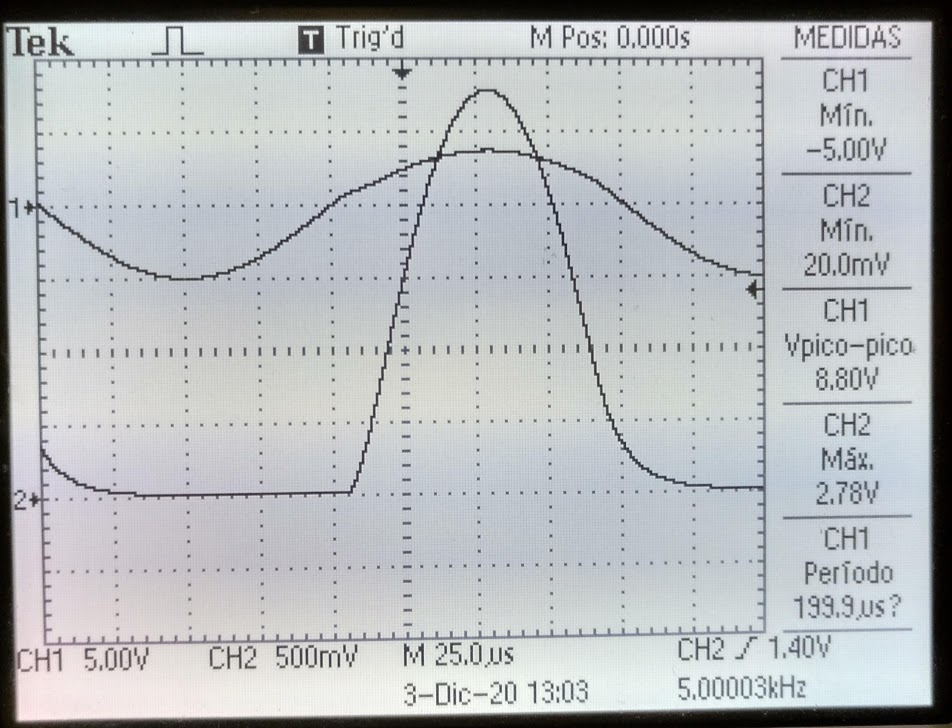
\includegraphics[scale=0.2]{100omega} 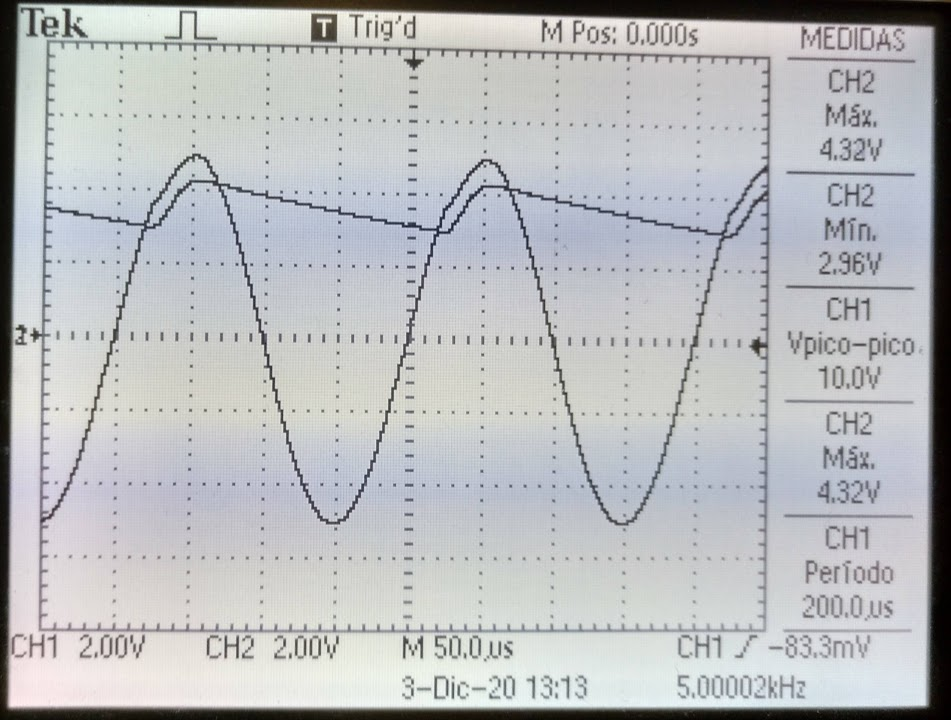
\includegraphics[scale=0.202]{4700omega}\\
Ondas correspondientes a Vout (junto con Vin), con $R_{load}=100\Omega$ (izquierda) y $R_{load}=4700\Omega$ (derecha).
\end{center}

Tabla de todos los valores:
\begin{table}[ht!]
\centering
\begin{tabular}{|r|r|r|r|r|}
\hline
\multicolumn{1}{|l|}{Rload $(\Omega)$} & \multicolumn{1}{l|}{Rload-valor real $(\Omega)$} & \multicolumn{1}{l|}{$V_{max}$ (V)} & \multicolumn{1}{l|}{$V_{min}$ (V)} & \multicolumn{1}{l|}{$V_{rizado}=V_{max}-V_{min}$, (V)} \\ \hline
100                                    & 98,5                                             & 2,76                               & 0,02                                                    & 2,74                         \\ \hline
220                                    & 218                                              & 3,44                               & 0,04                                                    & 3,4                          \\ \hline
470                                    & 466                                              & 3,84                               & 0,2                                                     & 3,64                         \\ \hline
1000                                   & 995                                              & 4,08                               & 0,88                                                    & 3,2                          \\ \hline
2200                                   & 2170                                             & 4,24                               & 2                                                       & 2,24                         \\ \hline
4700                                   & 4660                                             & 4,24                               & 2,96                                                    & 1,28                         \\ \hline
10000                                  & 9880                                             & 4,32                               & 3,6                                                     & 0,72                         \\ \hline
22000                                  & 21700                                            & 4,32                               & 4                                                       & 0,32                         \\ \hline
\end{tabular}
\end{table}

\bigskip
\textbf{c) Compare los resultados experimentales con los obtenidos en la simulación.}

Errores relativos en las medidas de (a) respecto a las de la simulación: 
$$V_{max, LTS} = 1,86V\Rightarrow E_{V_{max}}=100\times \frac{|1,86-1,86|}{1,86}=0\%$$
$$V_{min, LTS} = -1,37V\Rightarrow E_{V_{min}}=100\times \frac{|-1,56+1.37|}{|-1,37|}=13,9\%$$
$$V_{\gamma, LTS} = 0,67V\Rightarrow E_{V_{\gamma, 2}}=100\times \frac{|0,67-0,61|}{|0,67|}=8,9\%$$
$$E_{V_{\gamma, 3}}=100\times \frac{|0,67-0,86|}{|0,67|}=28,3\%$$

Estos valores varían un poco respecto a los medidos en la simulación, pero es posible que se deba a las pequeñas diferencias que puede haber entre los diodos, o que sus tensiones umbrales sean un poco distintas. Así como el resto de elementos del circuito y el riudo que puede entrar en el osciloscopio.

\bigskip
Comparación de los valores del apartado (b) respecto a la simulación de LTSpice, Circuito 2:

\begin{table}[ht!]
\centering
\begin{tabular}{|r|r|r|r|r|r|r|}
\hline
\multicolumn{1}{|l|}{Rload $(\Omega)$} & \multicolumn{1}{l|}{$V_{max}$ (V)} & \multicolumn{1}{l|}{$V_{max, LTS}$ (V)} & \multicolumn{1}{l|}{$E_{r,max}$} & \multicolumn{1}{l|}{$V_{min}$ (V)} & \multicolumn{1}{l|}{$V_{min, LTS}$ (V)} & \multicolumn{1}{l|}{$E_{r,min}$} \\ \hline
100                                    & 2,76                               & 4,24                                    & 34,91\%                                               & 0,02                                                    & 0                                       & \multicolumn{1}{c|}{-}           \\ \hline
220                                    & 3,44                               & 4,26                                    & 19,25\%                                               & 0,04                                                    & 0                                       & \multicolumn{1}{c|}{-}           \\ \hline
470                                    & 3,84                               & 4,29                                    & 10,49\%                                               & 0,2                                                     & 0,2                                     & 0,00\%                           \\ \hline
1000                                   & 4,08                               & 4,3                                     & 5,12\%                                                & 0,88                                                    & 0,93                                    & 5,38\%                           \\ \hline
2200                                   & 4,24                               & 4,32                                    & 1,85\%                                                & 2                                                       & 2,06                                    & 2,91\%                           \\ \hline
4700                                   & 4,24                               & 4,33                                    & 2,08\%                                                & 2,96                                                    & 3,01                                    & 1,66\%                           \\ \hline
10000                                  & 4,32                               & 4,35                                    & 0,69\%                                                & 3,6                                                     & 3,64                                    & 1,10\%                           \\ \hline
22000                                  & 4,32                               & 4,36                                    & 0,92\%                                                & 4                                                       & 4,01                                    & 0,25\%                           \\ \hline
\end{tabular}
\end{table}

Solamente hay variaciones significativas en $V_{max}$ en las resistencias de valores entre 100$\Omega$ y 1000$\Omega$. Para el resto de valores (tanto $V_{min}$ como $V_{max}$) los errores relativos son muy bajos, menores del 5\%, y según aumenta el valor de la resistencia, menor es el error relativo. No sé a qué se pueden deber estas variaciones para las resistencias bajas.

Las tensiones de rizado tienen valores también muy similares a los de la simulación:
\begin{table}[ht!]
\centering
\begin{tabular}{|r|r|r|r|}
\hline
\multicolumn{1}{|l|}{Rload $(\Omega)$} & \multicolumn{1}{l|}{$V_{rizado}$(V)} & \multicolumn{1}{l|}{$V_{rizado, LTS}$(V)} & \multicolumn{1}{l|}{$E_{r}$} \\ \hline
100                                    & 2,74                                                      & 4,24                                      & 35,38\%                                           \\ \hline
220                                    & 3,4                                                       & 4,26                                      & 20,19\%                                           \\ \hline
470                                    & 3,64                                                      & 4,09                                      & 11,00\%                                           \\ \hline
1000                                   & 3,2                                                       & 3,37                                      & 5,04\%                                            \\ \hline
2200                                   & 2,24                                                      & 2,26                                      & 0,88\%                                            \\ \hline
4700                                   & 1,28                                                      & 1,32                                      & 3,03\%                                            \\ \hline
10000                                  & 0,72                                                      & 0,71                                      & 1,41\%                                            \\ \hline
22000                                  & 0,32                                                      & 0,35                                      & 8,57\%                                            \\ \hline
\end{tabular}
\end{table}

\clearpage
\textbf{Utilice la fuente de alimentación DC para polarizar el Zener con V$^+$=5V y emplee una
resistencia R1=2,2k$\Omega$. No utilice la patilla del diodo etiquetada como ADJ.}

\bigskip
\begin{center}
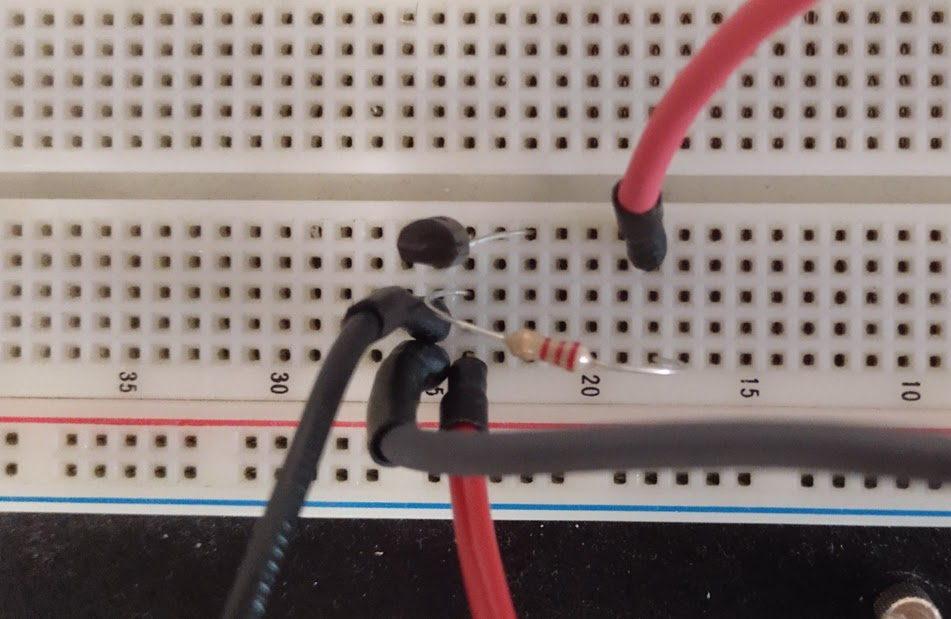
\includegraphics[scale=0.25]{c3}\\
Circuito montado con el diodo Zéner polarizado con la fuente de alimentación con 5V, en serie con la resistencia de 2,2k$\Omega$.
\end{center}

\bigskip
\textbf{d) Mida la tensión de salida Output con el voltímetro y observe cómo cambia cuando
cambia la temperatura del diodo Zener. El cambio tiene lugar en el rango de los mV
por lo que hay que utilizar la máxima precisión que proporcione el voltímetro.}

La salida inicial en el multímetro es de $2,97V$, y tras poner los dedos sobre el Zéner, para aumentar su temperatura llega a subir hasta $3,03V$.

\bigskip

\textbf{e) Teniendo en cuenta que el voltaje Zener aumenta unos 10 mV por grado, deduzca qué
temperatura tienen sus dedos con respecto al ambiente ¿Por qué no se mide la
temperatura tocando el termómetro con los dedos?}

El voltaje ha subido $60mV$ al poner los dedos, por lo que la temperatura ha aumentado unos 6 grados. Esto significa que si se midiera la temperatura corporal tocando el termómetro con los dedos se obtendría un valor mucho menor al que se tiene midiéndola correctamente. Ya que, suponiendo que la temperatura ambiente fuera de unos 20$^o$C, mis dedos habrían estado a unos 26$^o$C. Esto sería hasta 10 grados menor que mi temperatura corporal, que estaría al rededor de los 36,5$^o$C.

\end{document}
